\section{Appendix}
\appendix
\subsection{Effects of priors on $n'(r)$}
\begin{figure*}
  \begin{center}
    \hspace{-7mm}
    \includegraphics[width=0.3\textwidth]{fig/Gaia07_nr_bound/output/pdf/prof_nr_0.pdf}
    \includegraphics[width=0.3\textwidth]{fig/Gaia07_nr_bound/output/pdf/prof_rho_0.pdf}
    \includegraphics[width=0.3\textwidth]{fig/Gaia07_nr_bound/output/pdf/prof_beta_1.pdf}
  \end{center}
  \begin{center}
    \includegraphics[width=0.3\textwidth]{fig/Gaia07_nr_free/output/pdf/prof_nr_0.pdf}
    \includegraphics[width=0.3\textwidth]{fig/Gaia07_nr_free/output/pdf/prof_rho_0.pdf}
    \includegraphics[width=0.3\textwidth]{fig/Gaia07_nr_free/output/pdf/prof_beta_1.pdf}
  \end{center}
  \begin{center}
    \caption{Influence of $dn(r)/d\log r$ prior. The top panels show
      $n(r)$, $\rho(r)$, and $\beta^*(r)$ for Gaia07 with a moderate
      prior of $|dn(r)/d\log r|<1.5/(8/N_{\rm ipol})$, the lower
      panels show the same profiles with two times this value. We see
      that a tighter prior on $n(r)$ yields tighter constraints on $\beta^*$.}
    \label{fig:nrprime}
    \end{center}
\end{figure*}



\subsection{Convergence of the \MultiNest\ model ensemble}
We check the convergence of the MCMC twofold: first, the range of density
profiles swept after 5k, 50k and to the end of our run is increased from 5k to
50k, but stays approximately constant for another 16k runs, thus giving us
confidence that we found and fully explored the valid regions of phase space in
density. See fig. ~\ref{fig:convergencedens}.

\begin{figure*}
    \begin{center}
        \hspace{-7mm}
        %\includegraphics[width=0.3\textwidth]{fig/20130718132442_case_2_10000_0_cprior_nulog_denslog_mslope_rprior_5kits_profdens.pdf}
        %\includegraphics[width=0.3\textwidth]{fig/20130718132442_case_2_10000_0_cprior_nulog_denslog_mslope_rprior_50kits_profdens.pdf}
        %\includegraphics[width=0.3\textwidth]{fig/20130718132442_case_2_10000_0_cprior_nulog_denslog_mslope_rprior_67kits_profdens.pdf}
        \caption{\TODO{Convergence} of the density profile after
          (3k,30k,300k) iterations (left to right) for Gaia01.}
        \label{fig:convergencedens}
    \end{center}
\end{figure*}

% Second, the range of $\delta_i$, the only other unrestricted parameters, show
% a similar behaviour, as shown in ~\ref{fig:convergencedelta1} for $\delta_1$,
% with analogous $\delta_2$.
%
%\begin{figure*}
%    \begin{center}
%        \hspace{-7mm}
%        \includegraphics[width=0.3\textwidth]{fig/20130718132442_case_2_10000_0_cprior_nulog_denslog_mslope_rprior_5kit_profdelta1.pdf}
%        \includegraphics[width=0.3\textwidth]{fig/20130718132442_case_2_10000_0_cprior_nulog_denslog_mslope_rprior_50kit_profdelta1.pdf}
%        \includegraphics[width=0.3\textwidth]{fig/20130718132442_case_2_10000_0_cprior_nulog_denslog_mslope_rprior_67kit_profdelta1.pdf}
%        \caption{Convergence of $\delta_1$ after (5k,50k,67k) iterations (left to right).}
%        \label{fig:convergencedelta1}
%    \end{center}
%\end{figure*}
%

\subsection{The choice of binning}
\TODO{Consider the effect of varying the number of particles per bin for a single model.}
\TODO{explore different binning and lower sampling in an appendix}

%%% Local Variables:
%%% mode: latex
%%% TeX-master: "Steger_2014_Gravlite"
%%% End:
